取得した書き込める\chapter{主観評価におけるアプリケーション開発}
本章では、2.1節で述べた主観評価[参考文献]で利用するアプリケーションの概要と機能について説明する。これまでの主観評価実験では、遅延聴覚フィードバック下での違和感を被験者に実験者が用意した用紙に入力させ、その後PC上にデータを移行して結果を保存していた。このデータ移行には入力ミスのリスクがあり、注意深い作業が必要で研究にとって非効率であった。このアプリケーションを作成することで、被験者がアプリケーション上に直接評価結果を入力し、自動でcsvファイルに結果を出力できるようになる。これにより、実験者の負担が軽減され、効率的な実験および評価結果の分析が可能となり、短期間で多くの実験を実施することが期待できる。また,本アプリは,改善すべき点も多く残る.最後の節で改善すべき点について述べる.今後の開発者の改善に期待したい.
\section{アプリケーションの概要}
本研究では,Microsoft社が提供する統合開発環境であるMicrosoft Visual Studio 2022を使用し,C++で開発する.アプリケーションの外観を図3.1に示す.また,開発したアプリケーションのプログラムを付録Bに掲載する.以下に,開発するアプリケーションの機能を示す.
\begin{figure}[tbp]
  \centering
  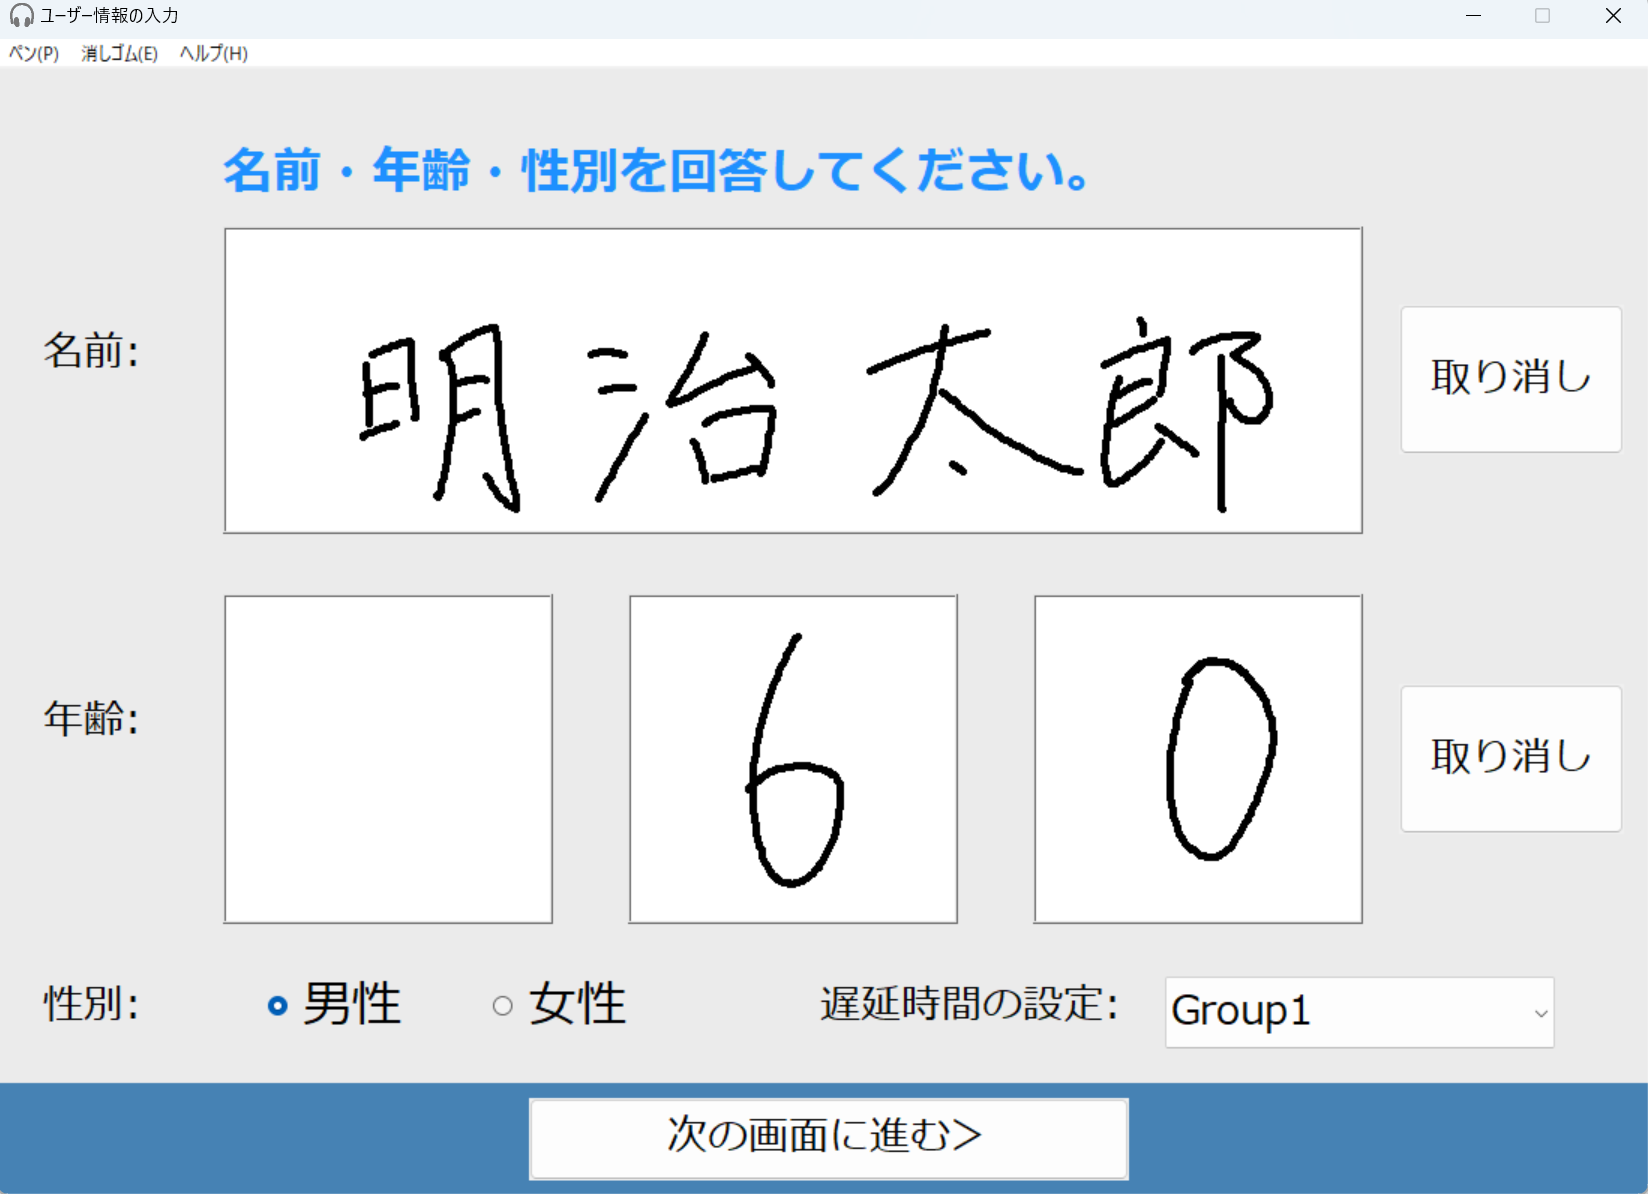
\includegraphics[scale=0.25]{figures/Syukann/gamen_1.png}
  \caption{最初の画面}
\end{figure}
\begin{figure}[tbp]
  \centering
  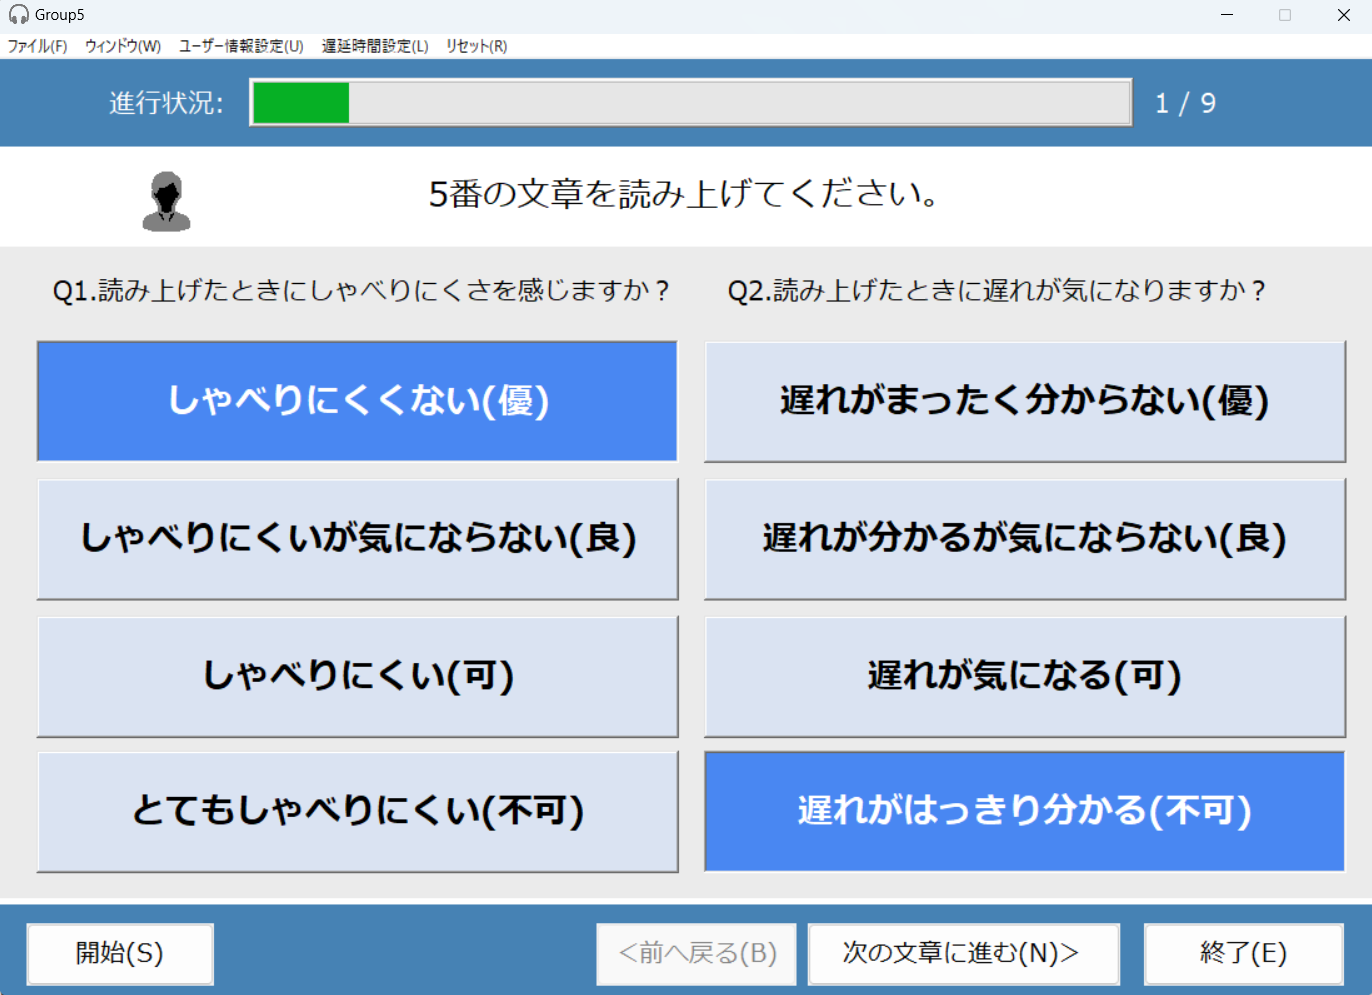
\includegraphics[scale=0.25]{figures/Syukann/app_2.png}
  \caption{2つ目の画面}
\end{figure}
\begin{enumerate}[leftmargin=*]
  \item 高齢者が使用することを想定し,タッチパネルのように名前と年齢を描画できる機能(3.1.1節参照)
  \item 被験者の名前と年齢,性別,遅延時間の設定が書かれている画面をキャプチャすると同時にそれらを外部ファイルに書き込む機能(3.1.2節参照)
  \item 読む文章の番号の順番をランダムに定義し,画面上に表示する機能
  \item 2つの質問に対するそれぞれ4つの回答項目をプッシュボタンとして表示し,押下された結果を(1)と同じ外部ファイルに書き込む機能(3.1.3節参照)
\end{enumerate}
(2)ではまず,random\_deviceクラスによりランダム数生成器を作成する.これをdefault\_random\_engineのシードとして使用し,デフォルトのランダムエンジンを初期化する.次に
\subsection{タッチパネルによるユーザー情報の取得}
指やペンなどの1つ以上のタッチポイントがタッチに依存するデジタイザーサーフェスに触れたときに,Windows APIの「WM\_TOUCH」メッセージがウィンドウに通知される.「WM\_TOUCH」イベントは,タッチ入力に関する情報を含んでおり,アプリケーションはこのイベントを処理して,タッチ操作に応じたアクションを実行することができる.このアクションには,例えばタッチするスクリーン上の位置,タッチの圧力,動きなどの情報が含まれる.このイベントを取り扱うためにまず,ウィンドウ作成時にRegisterTouchWindow()関数を使用してアプリケーションがタッチイベントを受けとることができるようにする.その後,ウィンドウプロージャで「WM\_TOUCH」メッセージ内の処理を行うことにより,タッチパネルとしての機能を実装する.「WM\_TOUCH」イベントが通知されたら以下の処理を行うように設定する.
\begin{enumerate}[leftmargin=*]
  \item ウィンドウのデバイスコンテキストのハンドルを取得し,デバイスコンテキストに新しいペンのハンドルを割り当てる.
  \item GetTouchInputInfo()関数を使用して,各タッチイベントの情報を取得する.
  \item 取得したタッチイベントの情報を元に,タッチポイントの座標を画面上の座標に変換し,タッチの位置がタッチパネル内にあるかどうかを確認する.タッチが続いている場合,以前のタッチポイントから現在のタッチポイントまで線を描画する.
  \item 各タッチポイントについて,前回のタッチポイントの位置とタッチパネルの内か外かを記録する.これにより,タッチの移動を追跡し,描画を連続的に行うことができるようにする.
  \item 描画が終わった後,使用したペンを削除し,デバイスコンテキストを解放する.
\end{enumerate}
\subsection{画面のキャプチャ}
図3.1に示したユーザーが手書きで入力した名前と年齢は,ウィンドウの画像を「次の画面に進む」というプッシュボタンをユーザーが押下したことを合図にウィンドウの画像をキャプチャし,JPEGファイルとして保存することによって記録する.画像をキャプチャする方法は,以下の手順で実装する.
\begin{enumerate}[leftmargin=*]
  \item GetDC()関数を使用して,ウィンドウのデバイスコンテキストを取得する.
  \item GetClientRect()関数を使用して,ウィンドウのクライアント領域の寸法を取得する.クライアント領域は,アプリケーションが描画できるウィンドウの部分であり,タイトルバーと境界線を除いた部分である.
  \item クライアント領域の幅と高さ,および年齢の100,10,1桁を表す3つの領域の幅と高さを計算する.
  \item CreateCompatibleDC()関数とCreateCompatibleBitmap()関数を使用して,ウィンドウ全体と3つの年齢を示す領域のメモリデバイスコンテキストおよびビットマップを作成する.
  \item BitBlt()関数を使用して,ウィンドウ全体と3つの年齢を示す領域のビットマップをメモリデバイスコンテキストにコピーする.
  \item c++のCImageクラスを使用して,ビットマップを読み込み.画像を指定したフォルダにJPEGとして保存される.そのフォルダが存在しない場合,新しく画像を保存するためのフォルダが作成される.
  \item 最後にCImageオブジェクトからビットマップを切り離し,ウィンドウのデバイスコンテキストを解放し,元のグラフィックオブジェクトをメモリデバイスコンテキストに再選択してから,ビットマップとメモリデバイスコンテキストを削除する.

\end{enumerate}
\subsection{回答の入力と出力}
2.1.1節において記述した主観調査では,「文章の読み上げ時のしゃべりにくさ」と「文章の読み上げ時の遅れの感じ方」に関する2つの質問が画面上に提示される.被験者は,これらの質問に対して,4つの選択肢の中からWindows APIにより実装したオーナーボタンを通じて回答する.ボタンが選択されると,背景色は青色に,文字色が白色になる設計となっており,これにより高齢者を含む操作に不慣れなユーザーでも,選択状態を直感的に把握できる.
また,背景色と文字色の変更は,ボタン押下時にInvalidRect()関数によって明示的にウィンドウの再描画を要求することによって実現している.ウィンドウの再描画が必要な場合,「WM\_ERASEBKGND」メッセージが受信され,ウィンドウの背景がクリアされた後,「WM\_PAINT」メッセージによってウィンドウの内容が再描画される.この2つの処理ステップが画面のちらつきを引き起こすことがあるため,「WM\_ERASEBKGND」メッセージの処理を明示的にスキップし,InvalidRect()で更新する領域を8つのボタンを含む領域の中で最小限に設定する.そうすることで,背景のクリア処理を行わずに直接「WM\_PAINT」メッセージでの再描画に移行する.これにより,背景と前景の描画が一度に行われるため,ちらつきを減少させることができ,特に高齢者にとって快適な操作体験が実現できる.

また,全てのボタンの選択状況を常に監視し,両方のボタンが選択されていない場合,「次の文章に進む」ボタンを無効化する.これにより,結果の記録における誤りを防止する.さらに,調査の進行状況を示すプログレスバーを画面上部に設置し,調査の進捗状況をユーザーに視覚的にフィードバックする.「次の文章に進む」ボタン押下時には音声信号が本プリケーションを起動しているデバイスから出力され,実験者はこの音声信号による合図を受けて,ユーザーの合図を待たずに次の調査へと移行できる.アンケート終了後,ユーザーが「次の文章に進む」ボタンを押下すると,アプリケーション起動時に選択したCSVファイルに,キャプチャした画面のハイパーリンク付き画像ファイルパス,遅延時間のグループ名,読まれた文章の番号,回答結果が自動的に記録される.既存のファイルであれば,結果はファイル末尾に追記される.このシステムにより,多数の被験者を対象とする実験でも,アプリケーションの再起動なしに迅速に実験を進行できるという利点がある.
% 改善すべき点
\section{今後の課題}
\begin{enumerate}
  \item 結果の出力.図のhyperlinkのとこ.excel以外で開くと文字化けする.
  \item 結果の出力.出力先ファイルが既に開かれていた場合,結果を書き込めなくなる.
\end{enumerate}
